
%(BEGIN_QUESTION)
% Copyright 2009, Tony R. Kuphaldt, released under the Creative Commons Attribution License (v 1.0)
% This means you may do almost anything with this work of mine, so long as you give me proper credit

Read and outline the ``Pneumatic Sensing Elements'' section of the ``Pneumatic Instrumentation'' chapter in your {\it Lessons In Industrial Instrumentation} textbook.  Note the page numbers where important illustrations, photographs, equations, tables, and other relevant details are found.  Prepare to thoughtfully discuss with your instructor and classmates the concepts and examples explored in this reading.


\underbar{file i03924}
%(END_QUESTION)





%(BEGIN_ANSWER)


%(END_ANSWER)





%(BEGIN_NOTES)

Baffle-and-nozzle mechanism used like a pneumatic pressure divider to cause a variable air pressure as a result of very small mechanical motion.  The baffle and nozzle form a variable restriction, while a fixed restriction (orifice) upstream serves as the other ``resistance'' in the divider network.  

\vskip 10pt

A similar principle is used in QC machined parts checking: proper fit of part into jig yields range of acceptable air pressures on a gauge.  Gauge indicates pass/fail test for part, without necessarily indicating air pressure in units such as PSI.






\vskip 20pt \vbox{\hrule \hbox{\strut \vrule{} {\bf Suggestions for Socratic discussion} \vrule} \hrule}

\begin{itemize}
\item{} Explain how a {\it flapper/nozzle} mechanism works.
\item{} Explain how the pneumatic quality-control checking jig works, and the {\it meaning} of the backpressure signal registered by the gauge.
\item{} If the supply air pressure on the quality-control test jig were doubled (from 20 PSI to 40 PSI), how would the operation of this device be affected (if at all)?
\item{} Does the depth of insertion affect the accuracy of the quality-control test jig?
\item{} Identify specific faults in a baffle-nozzle assembly that could cause the output air pressure to go {\it low}.
\item{} Identify specific faults in a baffle-nozzle assembly that could cause the output air pressure to go {\it high}.
\end{itemize}






















\vfil \eject

\noindent
{\bf Prep Quiz:}

Identify a condition that would cause the pressure gauge's indication to suddenly rise in this baffle/nozzle mechanism:

$$\includegraphics[width=15.5cm]{i03924x01.eps}$$


\begin{itemize}
\item{} The baffle moves further away from the nozzle
\vskip 5pt 
\item{} The nozzle develops a leak
\vskip 5pt 
\item{} The baffle moves sideways (to the left) 
\vskip 5pt 
\item{} The nozzle becomes plugged with debris
\vskip 5pt 
\item{} The baffle moves sideways (to the right)
\vskip 5pt 
\item{} The restriction becomes plugged with debris
\vskip 5pt 
\item{} The pressure gauge develops a leak
\end{itemize}



\vfil \eject

\noindent
{\bf Prep Quiz:}

Identify a condition that would cause the pressure gauge's indication to suddenly fall (decrease) in this baffle/nozzle mechanism:

$$\includegraphics[width=15.5cm]{i03924x01.eps}$$


\begin{itemize}
\item{} The baffle moves further away from the nozzle
\vskip 5pt 
\item{} The baffle moves closer to the nozzle
\vskip 5pt 
\item{} The baffle moves sideways (to the left) 
\vskip 5pt 
\item{} The nozzle becomes plugged with debris
\vskip 5pt 
\item{} The baffle moves sideways (to the right)
\vskip 5pt 
\item{} The supply pressure suddenly increases
\end{itemize}


%INDEX% Reading assignment: Lessons In Industrial Instrumentation, Pneumatic Instrumentation (pneumatic sensing elements)

%(END_NOTES)


